\section{Results}\label{sec:results}

\subsection{Learner models forecast equally well}\label{sec:res-forecast}

\Cref{tab:forecast} and \cref{fig:forecast} report first-attempt forecasts for the {{n_T}} test learners ({{n_predictions}} predictions). The six statistical models were practically indistinguishable: AUC ranged from {{auc_dkt2}} to {{auc_pfa}} and NLL varied by only {{nll_range}}, with PFA marginally best (NLL {{nll_pfa}}) and DKT at {{nll_dkt}}. The re-seeded DKT twin matched the original (NLL {{nll_dkt2}}). The pruned identification tree was less accurate (AUC {{auc_id3}}, NLL {{nll_id3}}) but produced readable rules; for example, a problem that fewer than 30\% of A learners passed, attempted by a learner whose overall first-attempt success was below 40\%, had a predicted success of about 0.09--0.10 across several skills. Skill-level discrimination was similar across models (\cref{tab:skills}); pointer problems had the lowest AUC and the fewest observations. Consistent with earlier comparisons \citep{khajah2016deep,wilson2016basics,gervet2020deep}, forecasting accuracy alone therefore provides no basis for preferring one of these models as a simulator.

\begin{table}[t]
\centering
\caption{First-attempt forecasts on held-out learners (models fitted on partition A).}
\label{tab:forecast}
\small
\resizebox{\linewidth}{!}{%
\begin{tabular}{lrcrcrr}
\toprule
Model & AUC & 95\% CI & NLL & 95\% CI & Brier & ECE \\
\midrule
{{table_forecast}}
\bottomrule
\end{tabular}}
\par\smallskip
\begin{minipage}{\linewidth}\footnotesize
\textit{Note.} CI: 95\% learner-bootstrap interval; NLL: negative log-likelihood; ECE: expected calibration error.
\end{minipage}
\end{table}

\begin{figure}[t]
\centering
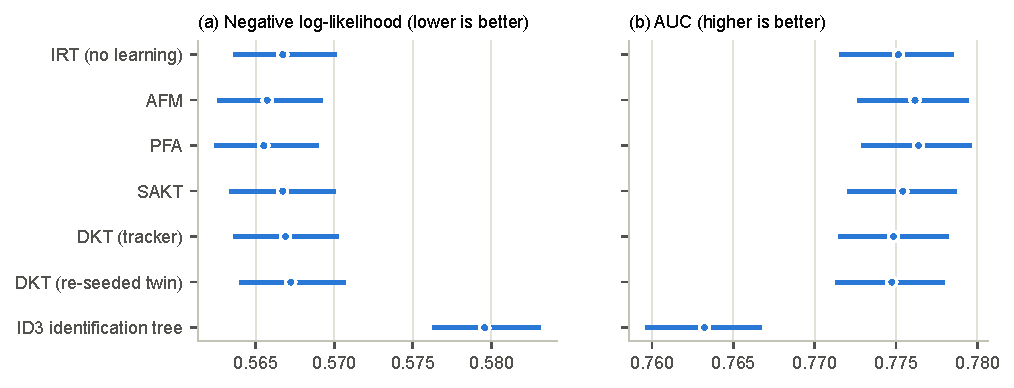
\includegraphics[width=\linewidth]{figures/fig_forecast.pdf}
\caption{Forecast accuracy on held-out learners. (a) Negative log-likelihood and (b) AUC of first-attempt forecasts for the {{n_T}} test learners ({{n_predictions}} predictions); bars are 95\% learner-bootstrap intervals. The six statistical learner models overlap; the interpretable identification tree is somewhat less accurate.}
\label{fig:forecast}
\end{figure}

\subsection{Policies look strong in the simulator they were trained in}\label{sec:res-insim}

In the training simulator DKT-A, the KT-reward agents produced the largest gains: PPO improved the expected post-test by {{insim_ppo_kt}} pp and DQN by {{insim_dqn_kt}} pp over ten problems, against {{insim_random}} pp for random selection; the one-step greedy maximiser of the tracker reached {{insim_greedy_kt}} pp (\cref{tab:matrix}). Agents trained in the AFM world or on mixed worlds also scored well in DKT-A (e.g.\ {{insim_dqn_mix}} pp for mixed-world DQN). Read in isolation, as is common in KT-simulator evaluations, these numbers would suggest a large benefit of reinforcement learning. They are, however, almost entirely drift: in DKT-A, where outcomes are generated by the tracker itself, the surprise term of \cref{eq:decomposition} averaged between {{insim_surprise_min}} and {{insim_surprise_max}} pp across the {{h3_n}} policies (at most {{insim_surprise_maxz}} Monte Carlo standard errors from zero; outcome streams are shared across policies), whereas PPO's accumulated drift was {{insim_drift_ppo_kt}} pp, as \cref{prop:insim} predicts (exploratory check).

\begin{table*}[t]
\centering
\caption{World-measured post-test gain (percentage points over ten problems) of every policy in every evaluation world.}
\label{tab:matrix}
\footnotesize
\resizebox{\textwidth}{!}{%
\begin{tabular}{{{matrix_cols}}}
\toprule
Policy & {{matrix_header}} \\
\midrule
{{table_matrix}}
\bottomrule
\end{tabular}}
\par\smallskip
\begin{minipage}{\textwidth}\footnotesize
\textit{Note.} Averages over {{episodes}} evaluation episodes and, for learned agents, three training seeds. $^\dagger$Training worlds. DKT and SAKT worlds are measured by their own predictions; AFM, PFA and ZPD worlds by the latent state; IRT-B has no learning, so every true gain is zero. The 95\% intervals are given in the supplementary file \texttt{evaluation\_matrix\_long.csv}.
\end{minipage}
\end{table*}

\subsection{H1: the in-simulator advantage does not survive independent worlds}\label{sec:res-h1}

Relative to random selection, DQN with the DKT reward gained {{dqn_kt_insim}} pp {{dqn_kt_insim_ci}} in DKT-A, but {{dqn_kt_adv_dkt2A}} pp in the re-seeded twin, {{dqn_kt_adv_dktB}} pp in DKT-B, {{dqn_kt_adv_saktB}} pp in SAKT-B, and {{dqn_kt_adv_afmB}}, {{dqn_kt_adv_pfaB}} and {{dqn_kt_adv_zpdB}} pp in the latent AFM-B, PFA-B and ZPD-B worlds. For PPO the in-simulator advantage was {{ppo_kt_insim}} pp {{ppo_kt_insim_ci}}, against {{ppo_kt_adv_dkt2A}}, {{ppo_kt_adv_dktB}}, {{ppo_kt_adv_saktB}}, {{ppo_kt_adv_afmB}}, {{ppo_kt_adv_pfaB}} and {{ppo_kt_adv_zpdB}} pp in the same six worlds. Every in-simulator-minus-independent difference was positive with an interval excluding zero (smallest: DQN versus the twin, {{dqn_kt_over_dkt2A}} pp {{dqn_kt_over_dkt2A_ci}}), supporting H1. In an exploratory comparison, policy rankings in DKT-A were only weakly related to rankings in the other worlds (Kendall $\tau$ = {{tau_dkt2A}} with the twin, {{tau_dktB}} with DKT-B, {{tau_saktB}} with SAKT-B, {{tau_afmB}} with AFM-B, {{tau_pfaB}} with PFA-B and {{tau_zpdB}} with ZPD-B). Neural worlds also disagreed with each other: the easy-to-hard curriculum gained {{gain_saktB_curriculum}} pp in SAKT-B but {{gain_dkt2A_curriculum}} pp in the DKT twin, where random selection gained {{gain_dkt2A_random}} pp (\cref{fig:matrix}).

\begin{figure}[t]
\centering
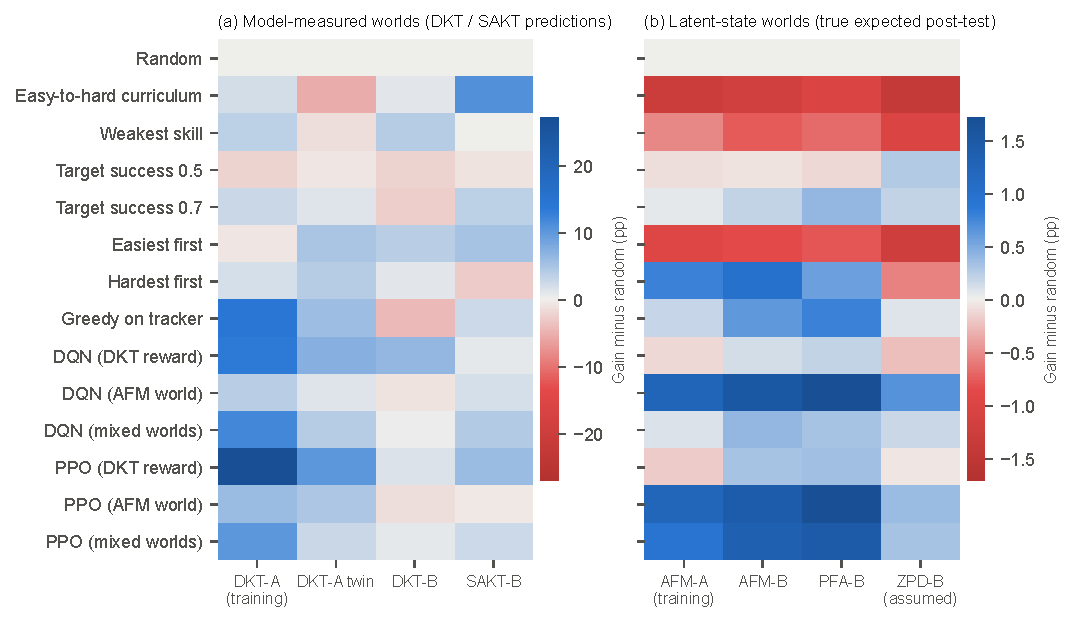
\includegraphics[width=\linewidth]{figures/fig_evaluation_matrix.pdf}
\caption{Gain relative to random selection in each world. (a) Worlds measured by a neural KT model's own predictions; (b) worlds with a known latent state. Blue cells: more simulated post-test gain than random; red cells: less. Colour scales differ between panels; values and 95\% intervals are in the supplementary file \texttt{evaluation\_matrix\_long.csv}.}
\label{fig:matrix}
\end{figure}

\subsection{H2 and H3: large gains are reported where no learning is possible}\label{sec:res-h2}

In the negative-control world IRT-B, the true post-test gain is exactly zero for every policy by construction. The deployed DKT tracker nevertheless reported gains of {{phantom_greedy_kt}} pp {{phantom_greedy_kt_ci}} for the greedy maximiser, {{phantom_dqn_kt}} pp {{phantom_dqn_kt_ci}} for DQN and {{phantom_ppo_kt}} pp {{phantom_ppo_kt_ci}} for PPO, supporting H2 (\cref{fig:phantom}). The reported gain depended strongly on the policy: it was {{phantom_random}} pp for random selection and {{phantom_dqn_afm}} pp for the AFM-trained DQN. Across the {{h3_n}} non-oracle policies, the gain in the training simulator and the phantom gain in the no-learning world were almost perfectly rank-correlated (Spearman $\rho$ = {{h3_rho}}), supporting H3 (\cref{fig:insim}): the ranking produced by the standard in-simulator evaluation is essentially the ranking of how much learning the tracker attributes to a policy's problem choices when there is none. Other models fitted on A were far less affected (exploratory; \cref{tab:observers}): in IRT-B, AFM and PFA reported gains of at most {{obs_afm_max}} and {{obs_pfa_max}} pp for any of these policies, and the static IRT model reported between {{obs_irt_min}} and {{obs_irt_max}} pp, that is, essentially none.

\begin{figure}[t]
\centering
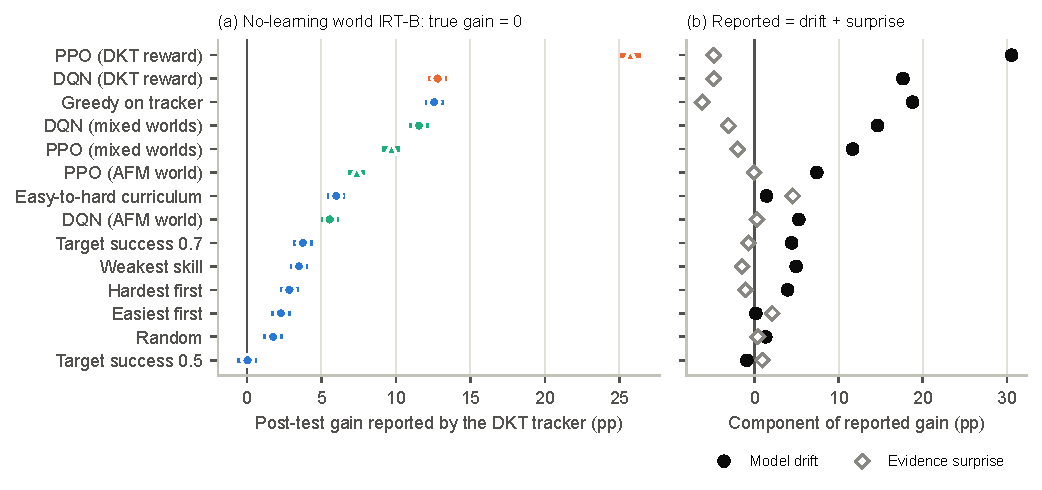
\includegraphics[width=\linewidth]{figures/fig_phantom_gain.pdf}
\caption{Negative control. (a) Post-test gain reported by the DKT tracker in the no-learning world IRT-B, where the true gain of every policy is zero (95\% intervals). (b) Exact decomposition of the reported gain into the tracker's drift and evidence surprise (\cref{eq:decomposition}).}
\label{fig:phantom}
\end{figure}

\begin{figure}[t]
\centering
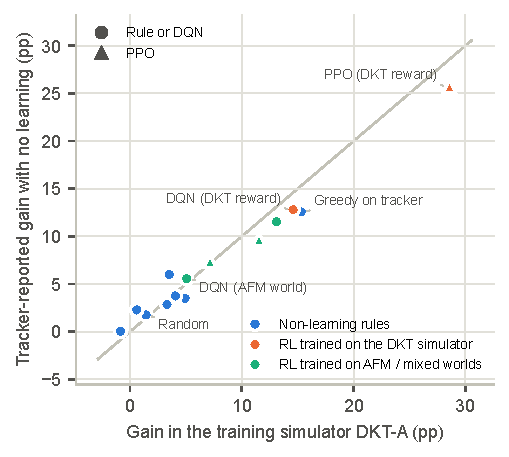
\includegraphics[width=0.62\linewidth]{figures/fig_in_sim_vs_phantom.pdf}
\caption{In-simulator gain in DKT-A against the phantom gain reported by the tracker in the no-learning world IRT-B for {{h3_n}} policies (Spearman $\rho$ = {{h3_rho}}). The grey diagonal is $y=x$; triangles are PPO agents.}
\label{fig:insim}
\end{figure}

\subsection{H4: where the phantom gain comes from}\label{sec:res-h4}

The decomposition in \cref{eq:decomposition} attributes the phantom gains to drift: in IRT-B, the tracker's own expected forecast change summed to {{drift_irt_ppo_kt}} pp for PPO, {{drift_irt_dqn_kt}} pp for DQN and {{drift_irt_greedy_kt}} pp for the greedy maximiser, partly offset by negative surprise because the world was less favourable than the tracker expected. The learning implied by a single practice problem was far more dispersed for the neural models than for the models with explicit learning terms (\cref{fig:implied}): the standard deviation of per-problem drift was {{sd_drift_dktA}} pp for DKT, {{sd_drift_dkt2A}} for its twin and {{sd_drift_saktA}} for SAKT, against {{sd_drift_afmA}} for AFM, {{sd_drift_pfaA}} for PFA and exactly {{sd_drift_irtA}} for IRT, as \cref{prop:nodrift} requires. The DKT--AFM difference was {{h4}} pp {{h4_ci}}, supporting H4. In exploratory analyses, the two DKTs, which forecast equally well, agreed only weakly on which problems ``teach'' (Spearman $\rho$ = {{twin_rho}} {{twin_rho_ci}}), and DKT drift was higher for frequently attempted problems ($\rho$ = {{expl_support_fraction}}) and for easier problems ($\rho$ = {{expl_irt_difficulty}} with IRT difficulty) but unrelated to typical course position ($\rho$ = {{expl_course_position}}).

Along learners' own next ten real interactions ({{lc_n}} learners; exploratory), the tracker's post-test forecast moved on average by only {{lc_tracker_gain}} pp, although the absolute movement averaged {{lc_tracker_gain_abs}} pp, compared with {{lc_claimed_irt_A_abs}} pp for IRT. On the sequences that learners actually followed, DKT's drift therefore largely cancels out; only when a policy selects problems for their drift does it accumulate into double-digit gains.

\begin{figure}[t]
\centering
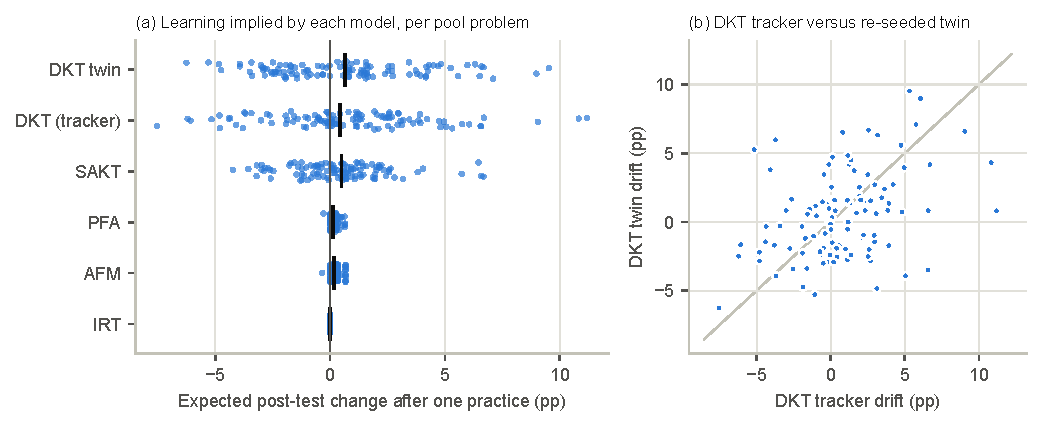
\includegraphics[width=\linewidth]{figures/fig_implied_learning.pdf}
\caption{Learning implied by each model. (a) Expected post-test change after one practice of each pool problem (drift), averaged over 300 start states; vertical bars are medians. (b) Drift of the DKT tracker against its re-seeded twin (Spearman $\rho$ = {{twin_rho}}); the grey diagonal is $y=x$.}
\label{fig:implied}
\end{figure}

\subsection{Exploratory: which policies transfer}\label{sec:res-latent}

In the latent-state worlds the spread between policies was small but consistent (\cref{fig:effort}). Agents trained in the AFM world were the best non-privileged policies: in AFM-B the AFM-trained DQN gained {{gain_afmB_dqn_afm}} pp and PPO {{gain_afmB_ppo_afm}} pp, against {{gain_afmB_random}} pp for random and {{gain_afmB_oracle}} pp for the privileged one-step oracle; in PFA-B the corresponding values were {{gain_pfaB_dqn_afm}}, {{gain_pfaB_ppo_afm}}, {{gain_pfaB_random}} and {{gain_pfaB_oracle}} pp. In the assumed desirable-difficulty world ZPD-B the margin was smaller ({{gain_zpdB_dqn_afm}} and {{gain_zpdB_ppo_afm}} against {{gain_zpdB_random}} pp). Their worst-case advantage over random across the three latent worlds was {{wc_dqn_afm}} pp for DQN and {{wc_ppo_afm}} pp for PPO, the largest of all policies, whereas the KT-reward agents had worst cases of {{wc_dqn_kt}} and {{wc_ppo_kt}} pp; PPO trained on mixed worlds came close ({{wc_ppo_mix}} pp). The AFM-trained agents also needed fewer extra submissions ({{extra_afmB_dqn_afm}} and {{extra_afmB_ppo_afm}} per ten problems in AFM-B, against {{extra_afmB_random}} for random).

This robustness has a clear limit. AFM-B, PFA-B and ZPD-B share the additive logistic structure of the AFM training world, so transfer among them is partly by construction. In the neural worlds, which do not share that structure, the AFM-trained agents' advantage over random ranged from {{rob_min_neural_afm}} to {{rob_max_neural_afm}} pp and was negative in DKT-B ({{rob_dqn_afm_dktB}} and {{rob_ppo_afm_dktB}} pp). Rules that targeted a predicted success of 0.7 were slightly better than random in every latent world (worst case {{wc_zpd70}} pp), whereas the easy-to-hard curriculum and easiest-first rules were consistently the worst in the latent worlds, spending practice on problems the learner would already solve.

\begin{figure}[t]
\centering
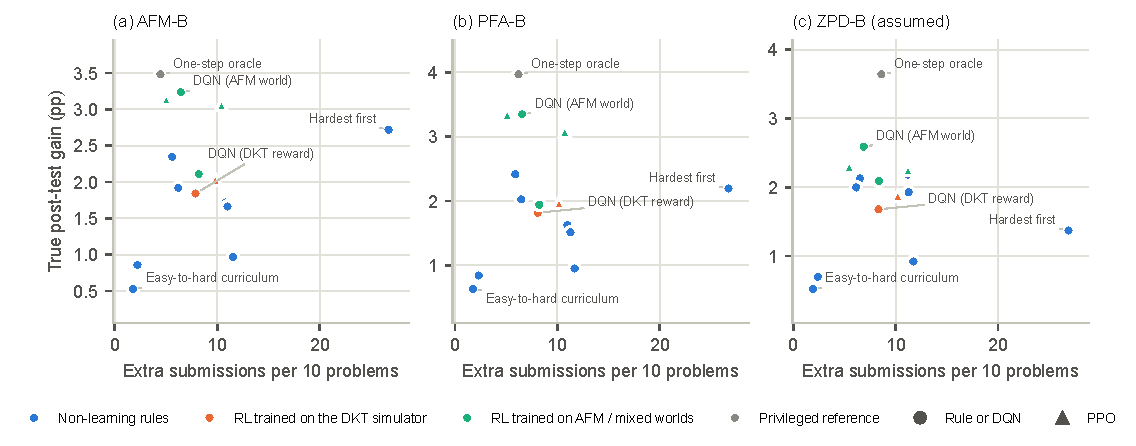
\includegraphics[width=\linewidth]{figures/fig_gain_effort.pdf}
\caption{True post-test gain against extra submissions per ten problems in the three latent worlds fitted or constructed from partition B: (a) AFM-B, (b) PFA-B and (c) the assumed desirable-difficulty world ZPD-B. Colours distinguish policy families and triangles mark PPO agents.}
\label{fig:effort}
\end{figure}
